\documentclass[tikz,border=8pt]{standalone}
% Shared preamble for the bootqcc TikZ figures.
\usepackage[T1]{fontenc}
\usepackage{helvet}
\renewcommand{\familydefault}{\sfdefault}
\usepackage{amsmath}
\usetikzlibrary{arrows.meta,positioning,shapes.geometric,fit,backgrounds,calc}

\definecolor{navy}{HTML}{1F3A5F}
\definecolor{sky}{HTML}{5AA9E6}
\definecolor{coral}{HTML}{FF6B6B}
\definecolor{slate}{HTML}{6B7A8F}

\tikzset{
  box/.style={rectangle, rounded corners=4pt, draw=navy, fill=sky!15, thick,
              align=center, minimum height=1.0cm, inner sep=6pt, text width=4.6cm},
  inbox/.style={rectangle, rounded corners=4pt, draw=slate, fill=slate!10, thick,
              align=center, minimum height=0.9cm, inner sep=5pt, text width=3.0cm,
              font=\small},
  io/.style={trapezium, trapezium left angle=72, trapezium right angle=108,
             draw=navy, fill=white, thick, align=center, minimum height=1.2cm,
             inner sep=5pt, text width=3.0cm},
  result/.style={rectangle, rounded corners=8pt, draw=coral, fill=coral!10, thick,
              align=center, minimum height=1.0cm, inner sep=6pt, text width=4.0cm},
  term/.style={rectangle, rounded corners=12pt, draw=navy, fill=navy, text=white,
               thick, align=center, minimum height=0.9cm, inner sep=6pt, text width=4.2cm},
  dec/.style={diamond, aspect=2.6, draw=navy, fill=white, thick, align=center,
              inner sep=0pt, text width=2.7cm, font=\small},
  err/.style={rectangle, rounded corners=4pt, draw=coral, fill=coral!15, thick,
              align=center, minimum height=0.9cm, inner sep=6pt, text width=3.2cm},
  arr/.style={-{Latex[length=3mm]}, thick, navy},
  lab/.style={font=\footnotesize\bfseries, text=navy, fill=white, inner sep=1.5pt},
  phase/.style={rounded corners=8pt, draw=navy!45, dashed, thick, inner sep=12pt},
}

\begin{document}
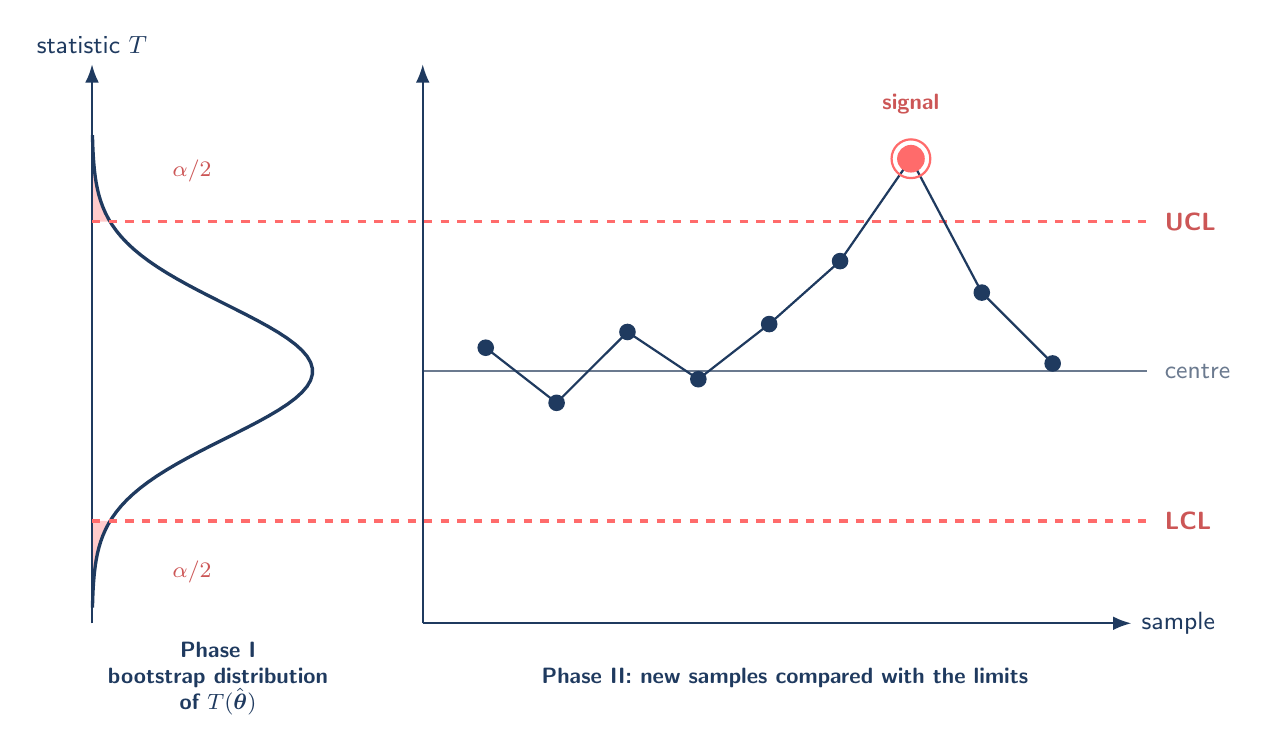
\begin{tikzpicture}[x=1cm,y=1cm]

  % ---- Phase I: bootstrap distribution of the statistic (sideways) ----
  \def\mu{3.0}\def\sg{0.85}\def\dw{2.8}
  % tails beyond the alpha/2 quantiles
  \fill[coral!35] (0,{\mu+1.9}) -- plot[domain={\mu+1.9}:{\mu+3.0}, samples=30, variable=\y]
        ({\dw*exp(-(\y-\mu)*(\y-\mu)/(2*\sg*\sg))},\y) -- (0,{\mu+3.0}) -- cycle;
  \fill[coral!35] (0,{\mu-1.9}) -- plot[domain={\mu-1.9}:{\mu-3.0}, samples=30, variable=\y]
        ({\dw*exp(-(\y-\mu)*(\y-\mu)/(2*\sg*\sg))},\y) -- (0,{\mu-3.0}) -- cycle;
  \draw[navy, very thick, domain={\mu-3.0}:{\mu+3.0}, samples=80, variable=\y]
        plot ({\dw*exp(-(\y-\mu)*(\y-\mu)/(2*\sg*\sg))},\y);
  \draw[navy, thick, -{Latex}] (0,-0.2) -- (0,6.9) node[above, font=\small] {statistic $T$};
  \node[navy, font=\footnotesize\bfseries, align=center] at (1.6,-0.9)
        {Phase I\\ bootstrap distribution\\ of $T(\hat{\boldsymbol\theta})$};
  \node[coral!80!black, font=\footnotesize, anchor=west] at (0.9,{\mu+2.55}) {$\alpha/2$};
  \node[coral!80!black, font=\footnotesize, anchor=west] at (0.9,{\mu-2.55}) {$\alpha/2$};

  % ---- control limits carried over to the chart ----
  \def\ucl{4.9}\def\lcl{1.1}
  \draw[coral, very thick, dashed] (0,\ucl) -- (13.4,\ucl);
  \draw[coral, very thick, dashed] (0,\lcl) -- (13.4,\lcl);
  \draw[slate, thick] (4.2,\mu) -- (13.4,\mu);
  \node[coral!80!black, font=\small\bfseries, anchor=west] at (13.5,\ucl) {UCL};
  \node[coral!80!black, font=\small\bfseries, anchor=west] at (13.5,\lcl) {LCL};
  \node[slate, font=\small, anchor=west] at (13.5,\mu) {centre};

  % ---- Phase II chart ----
  \draw[navy, thick, -{Latex}] (4.2,-0.2) -- (13.2,-0.2) node[right, font=\small] {sample};
  \draw[navy, thick, -{Latex}] (4.2,-0.2) -- (4.2,6.9);
  \node[navy, font=\footnotesize\bfseries] at (8.8,-0.9) {Phase II: new samples compared with the limits};

  \coordinate (p1) at (5.0,3.3);
  \coordinate (p2) at (5.9,2.6);
  \coordinate (p3) at (6.8,3.5);
  \coordinate (p4) at (7.7,2.9);
  \coordinate (p5) at (8.6,3.6);
  \coordinate (p6) at (9.5,4.4);
  \coordinate (p7) at (10.4,5.7);
  \coordinate (p8) at (11.3,4.0);
  \coordinate (p9) at (12.2,3.1);
  \draw[navy, thick] (p1)--(p2)--(p3)--(p4)--(p5)--(p6)--(p7)--(p8)--(p9);
  \foreach \p in {p1,p2,p3,p4,p5,p6,p8,p9} \fill[navy] (\p) circle (3pt);
  \fill[coral] (p7) circle (5pt);
  \draw[coral, thick] (p7) circle (7pt);
  \node[coral!80!black, font=\footnotesize\bfseries, anchor=south] at ($(p7)+(0,0.45)$) {signal};

\end{tikzpicture}
\end{document}
